

% Gradient Info

\tikzset {_2zcujs10x/.code = {\pgfsetadditionalshadetransform{ \pgftransformshift{\pgfpoint{228 bp } { -600 bp }  }  \pgftransformscale{3 }  }}}
\pgfdeclareradialshading{_gt23p819p}{\pgfpoint{-80bp}{232bp}}{rgb(0bp)=(0.96,0.96,0.96);
	rgb(0bp)=(0.96,0.96,0.96);
	rgb(5.25bp)=(0.86,0.86,0.89);
	rgb(12.25bp)=(0.72,0.73,0.78);
	rgb(20bp)=(0.87,0.87,0.89);
	rgb(25bp)=(0.96,0.96,0.96);
	rgb(400bp)=(0.96,0.96,0.96)}

% Gradient Info

\tikzset {_ke7fkjhbt/.code = {\pgfsetadditionalshadetransform{ \pgftransformshift{\pgfpoint{0 bp } { 0 bp }  }  \pgftransformrotate{0 }  \pgftransformscale{2 }  }}}
\pgfdeclarehorizontalshading{_zhaeh0lf2}{150bp}{rgb(0bp)=(1,1,1);
	rgb(61.622025626046316bp)=(1,1,1);
	rgb(62.5bp)=(0.9,0.9,0.9);
	rgb(100bp)=(0.9,0.9,0.9)}

% Gradient Info

\tikzset {_ivori3i8z/.code = {\pgfsetadditionalshadetransform{ \pgftransformshift{\pgfpoint{-6 bp } { 4.5 bp }  }  \pgftransformrotate{0 }  \pgftransformscale{6 }  }}}
\pgfdeclarehorizontalshading{_nhbclds00}{150bp}{rgb(0bp)=(0.96,0.96,0.96);
	rgb(37.5bp)=(0.96,0.96,0.96);
	rgb(42.75bp)=(0.86,0.86,0.89);
	rgb(49.75bp)=(0.72,0.73,0.78);
	rgb(57.5bp)=(0.87,0.87,0.89);
	rgb(62.5bp)=(0.96,0.96,0.96);
	rgb(100bp)=(0.96,0.96,0.96)}

% Gradient Info

\tikzset {_jlfrhqr83/.code = {\pgfsetadditionalshadetransform{ \pgftransformshift{\pgfpoint{-6 bp } { 4.5 bp }  }  \pgftransformrotate{0 }  \pgftransformscale{6 }  }}}
\pgfdeclarehorizontalshading{_icebnqz8w}{150bp}{rgb(0bp)=(0.96,0.96,0.96);
	rgb(37.5bp)=(0.96,0.96,0.96);
	rgb(42.75bp)=(0.86,0.86,0.89);
	rgb(49.75bp)=(0.72,0.73,0.78);
	rgb(57.5bp)=(0.87,0.87,0.89);
	rgb(62.5bp)=(0.96,0.96,0.96);
	rgb(100bp)=(0.96,0.96,0.96)}
\tikzset{every picture/.style={line width=0.75pt}} %set default line width to 0.75pt        

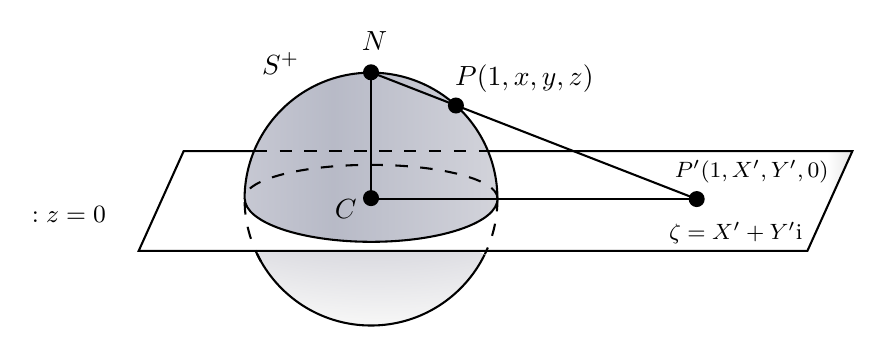
\begin{tikzpicture}[x=0.75pt,y=0.75pt,yscale=-1,xscale=1]
	%uncomment if require: \path (0,152); %set diagram left start at 0, and has height of 152
	
	%Shape: Arc [id:dp7778812556944477] 
	\draw  [draw opacity=0][shading=_gt23p819p,_2zcujs10x] (352.66,112.84) .. controls (342.75,133.07) and (321.96,147) .. (297.92,147) .. controls (273.72,147) and (252.81,132.89) .. (242.99,112.45) -- (297.92,86.08) -- cycle ; \draw   (352.66,112.84) .. controls (342.75,133.07) and (321.96,147) .. (297.92,147) .. controls (273.72,147) and (252.81,132.89) .. (242.99,112.45) ;  
	%Shape: Parallelogram [id:dp14729101837402525] 
	\path  [shading=_zhaeh0lf2,_ke7fkjhbt] (207.64,63) -- (529.83,63) -- (508.19,111) -- (186,111) -- cycle ; % for fading 
	\draw   (207.64,63) -- (529.83,63) -- (508.19,111) -- (186,111) -- cycle ; % for border 
	
	%Shape: Arc [id:dp009547815145512395] 
	\draw  [draw opacity=0][dash pattern={on 4.5pt off 4.5pt}] (358.83,86.02) .. controls (358.83,86.04) and (358.83,86.06) .. (358.83,86.08) .. controls (358.83,95.59) and (356.65,104.59) .. (352.77,112.61) -- (297.92,86.08) -- cycle ; \draw  [dash pattern={on 4.5pt off 4.5pt}] (358.83,86.02) .. controls (358.83,86.04) and (358.83,86.06) .. (358.83,86.08) .. controls (358.83,95.59) and (356.65,104.59) .. (352.77,112.61) ;  
	%Shape: Arc [id:dp2605619902920453] 
	\draw  [draw opacity=0][dash pattern={on 4.5pt off 4.5pt}] (244.93,116.16) .. controls (239.88,107.29) and (237,97.02) .. (237,86.08) .. controls (237,84.97) and (237.03,83.86) .. (237.09,82.76) -- (297.92,86.08) -- cycle ; \draw  [dash pattern={on 4.5pt off 4.5pt}] (244.93,116.16) .. controls (239.88,107.29) and (237,97.02) .. (237,86.08) .. controls (237,84.97) and (237.03,83.86) .. (237.09,82.76) ;  
	%Shape: Arc [id:dp014360101618336563] 
	\draw  [draw opacity=0][shading=_nhbclds00,_ivori3i8z] (237,86.14) .. controls (237,86.12) and (237,86.1) .. (237,86.08) .. controls (237,52.44) and (264.27,25.17) .. (297.92,25.17) .. controls (331.43,25.17) and (358.63,52.23) .. (358.83,85.7) -- (297.92,86.08) -- cycle ; \draw   (237,86.14) .. controls (237,86.12) and (237,86.1) .. (237,86.08) .. controls (237,52.44) and (264.27,25.17) .. (297.92,25.17) .. controls (331.43,25.17) and (358.63,52.23) .. (358.83,85.7) ;  
	%Shape: Arc [id:dp5813015502811212] 
	\draw  [draw opacity=0][shading=_icebnqz8w,_jlfrhqr83] (358.92,85.75) .. controls (358.92,85.77) and (358.92,85.8) .. (358.92,85.83) .. controls (358.92,97.34) and (331.65,106.67) .. (298,106.67) .. controls (264.36,106.67) and (237.09,97.34) .. (237.09,85.83) .. controls (237.09,85.81) and (237.09,85.78) .. (237.09,85.76) -- (298,85.83) -- cycle ; \draw   (358.92,85.75) .. controls (358.92,85.77) and (358.92,85.8) .. (358.92,85.83) .. controls (358.92,97.34) and (331.65,106.67) .. (298,106.67) .. controls (264.36,106.67) and (237.09,97.34) .. (237.09,85.83) .. controls (237.09,85.81) and (237.09,85.78) .. (237.09,85.76) ;  
	%Straight Lines [id:da5221405117017395] 
	\draw  [dash pattern={on 4.5pt off 4.5pt}]  (241.83,63) -- (353.83,63) ;
	%Straight Lines [id:da24524464444311378] 
	\draw    (297.92,25) -- (454.83,86.08) ;
	%Shape: Arc [id:dp550601865905674] 
	\draw  [draw opacity=0][dash pattern={on 4.5pt off 4.5pt}] (358.83,85.7) .. controls (358.83,85.67) and (358.83,85.64) .. (358.83,85.62) .. controls (358.83,76.76) and (331.56,69.59) .. (297.92,69.59) .. controls (264.27,69.59) and (237,76.76) .. (237,85.62) .. controls (237,85.64) and (237,85.67) .. (237,85.69) -- (297.92,85.62) -- cycle ; \draw  [dash pattern={on 4.5pt off 4.5pt}] (358.83,85.7) .. controls (358.83,85.67) and (358.83,85.64) .. (358.83,85.62) .. controls (358.83,76.76) and (331.56,69.59) .. (297.92,69.59) .. controls (264.27,69.59) and (237,76.76) .. (237,85.62) .. controls (237,85.64) and (237,85.67) .. (237,85.69) ;  
	%Straight Lines [id:da047382324055451175] 
	\draw    (297.92,86.08) -- (454.83,86.08) ;
	\draw [shift={(454.83,86.08)}, rotate = 0] [color={rgb, 255:red, 0; green, 0; blue, 0 }  ][fill={rgb, 255:red, 0; green, 0; blue, 0 }  ][line width=0.75]      (0, 0) circle [x radius= 3.35, y radius= 3.35]   ;
	%Straight Lines [id:da4398538993246077] 
	\draw    (297.92,25) -- (297.92,85.62) ;
	\draw [shift={(297.92,85.62)}, rotate = 90] [color={rgb, 255:red, 0; green, 0; blue, 0 }  ][fill={rgb, 255:red, 0; green, 0; blue, 0 }  ][line width=0.75]      (0, 0) circle [x radius= 3.35, y radius= 3.35]   ;
	\draw [shift={(297.92,25)}, rotate = 90] [color={rgb, 255:red, 0; green, 0; blue, 0 }  ][fill={rgb, 255:red, 0; green, 0; blue, 0 }  ][line width=0.75]      (0, 0) circle [x radius= 3.35, y radius= 3.35]   ;
	%Straight Lines [id:da9917829639130094] 
	\draw    (338.83,41) ;
	\draw [shift={(338.83,41)}, rotate = 0] [color={rgb, 255:red, 0; green, 0; blue, 0 }  ][fill={rgb, 255:red, 0; green, 0; blue, 0 }  ][line width=0.75]      (0, 0) circle [x radius= 3.35, y radius= 3.35]   ;
	
	
	% Text Node
	\draw (440,95.96) node [anchor=north west][inner sep=0.75pt]  [font=\footnotesize]  {$\zeta =X'+Y'\mathrm{i}$};
	% Text Node
	\draw (133,88) node [anchor=north west][inner sep=0.75pt]  [font=\small]  {$\upSigma :z=0$};
	% Text Node
	\draw (244,14) node [anchor=north west][inner sep=0.75pt]    {$S^{+}$};
	% Text Node
	\draw (292,4) node [anchor=north west][inner sep=0.75pt]    {$N$};
	% Text Node
	\draw (337,20) node [anchor=north west][inner sep=0.75pt]    {$P( 1,x,y,z)$};
	% Text Node
	\draw (279,85) node [anchor=north west][inner sep=0.75pt]    {$C$};
	% Text Node
	\draw (442.83,66.08) node [anchor=north west][inner sep=0.75pt]  [font=\footnotesize]  {$P'( 1,X',Y',0)$};
	
	
\end{tikzpicture}